
The Scottish Highlands and Islands consist of mountainous  terrain stretching 400km North to South consisting of islands in the West together with deep lochs and glens penetrating the mainland to the East.  The economy was traditionally maritime, and nearly all habitation is at sea level or in the glens.  

Until recently there was little fibre in the region.  Many exchanges were served by microwave links. That has started to change, but the main problem remains that the fibre reaches only to exchanges; and fibre-based services are available at only a few of them.  Many communities rely on copper connections to those exchanges in excess of 5km, and there is little prospect of replacing that copper.  In the medium term future local wireless distribution offers the only feasible technology for adequate bandwidth and quality of service\footnote{There is often no mobile reception, and some sites cannot "see" satellites.}.

Starting in 2008, the Tegola project~\cite{tegola} started to experiment with technology that would enable communities to build their own wireless distribution networks.  This included electrical and mechanical infrastructure as well as wireless equipment.  It rapidly became clear that volunteer communities or small businesses could construct and maintain these networks at a small fraction of the cost that a centralized organizaton would charge for a number of reasons: first, the cost and time of travel to service the relays in remote areas is infinitessimal compared with the cost of a helicopter; second site licences and wayleaves can usually be negotiated for free by lightweight agreements; third, we have developed basic technology (Fig. \ref{fig:mhialairigh}) for robust, inexpensive relay construction that works well in the mountainous terrain in which the project operates\footnote{See \url{www.tegola.org.uk}}.

 The ideas were taken up by a number of communities across Scotland including those around the Tegola project shown in Figure ~\ref{fig:whixmap}, which extend over 100km of the coastline. A typical community would have a local distribution network and point-to-point links, often in excess of 20km, connected to a (possibly bonded) set of ADSL lines somewhere near a telephone exchange. This was far from ideal, but it was the only affordable source of backhaul. Although the communities shared their expertise and sometimes their infrastructure, they operated independently.
%% figure as opposed to figure* just in interests of space
%%Thanks
\begin{figure}[h]
\centering
 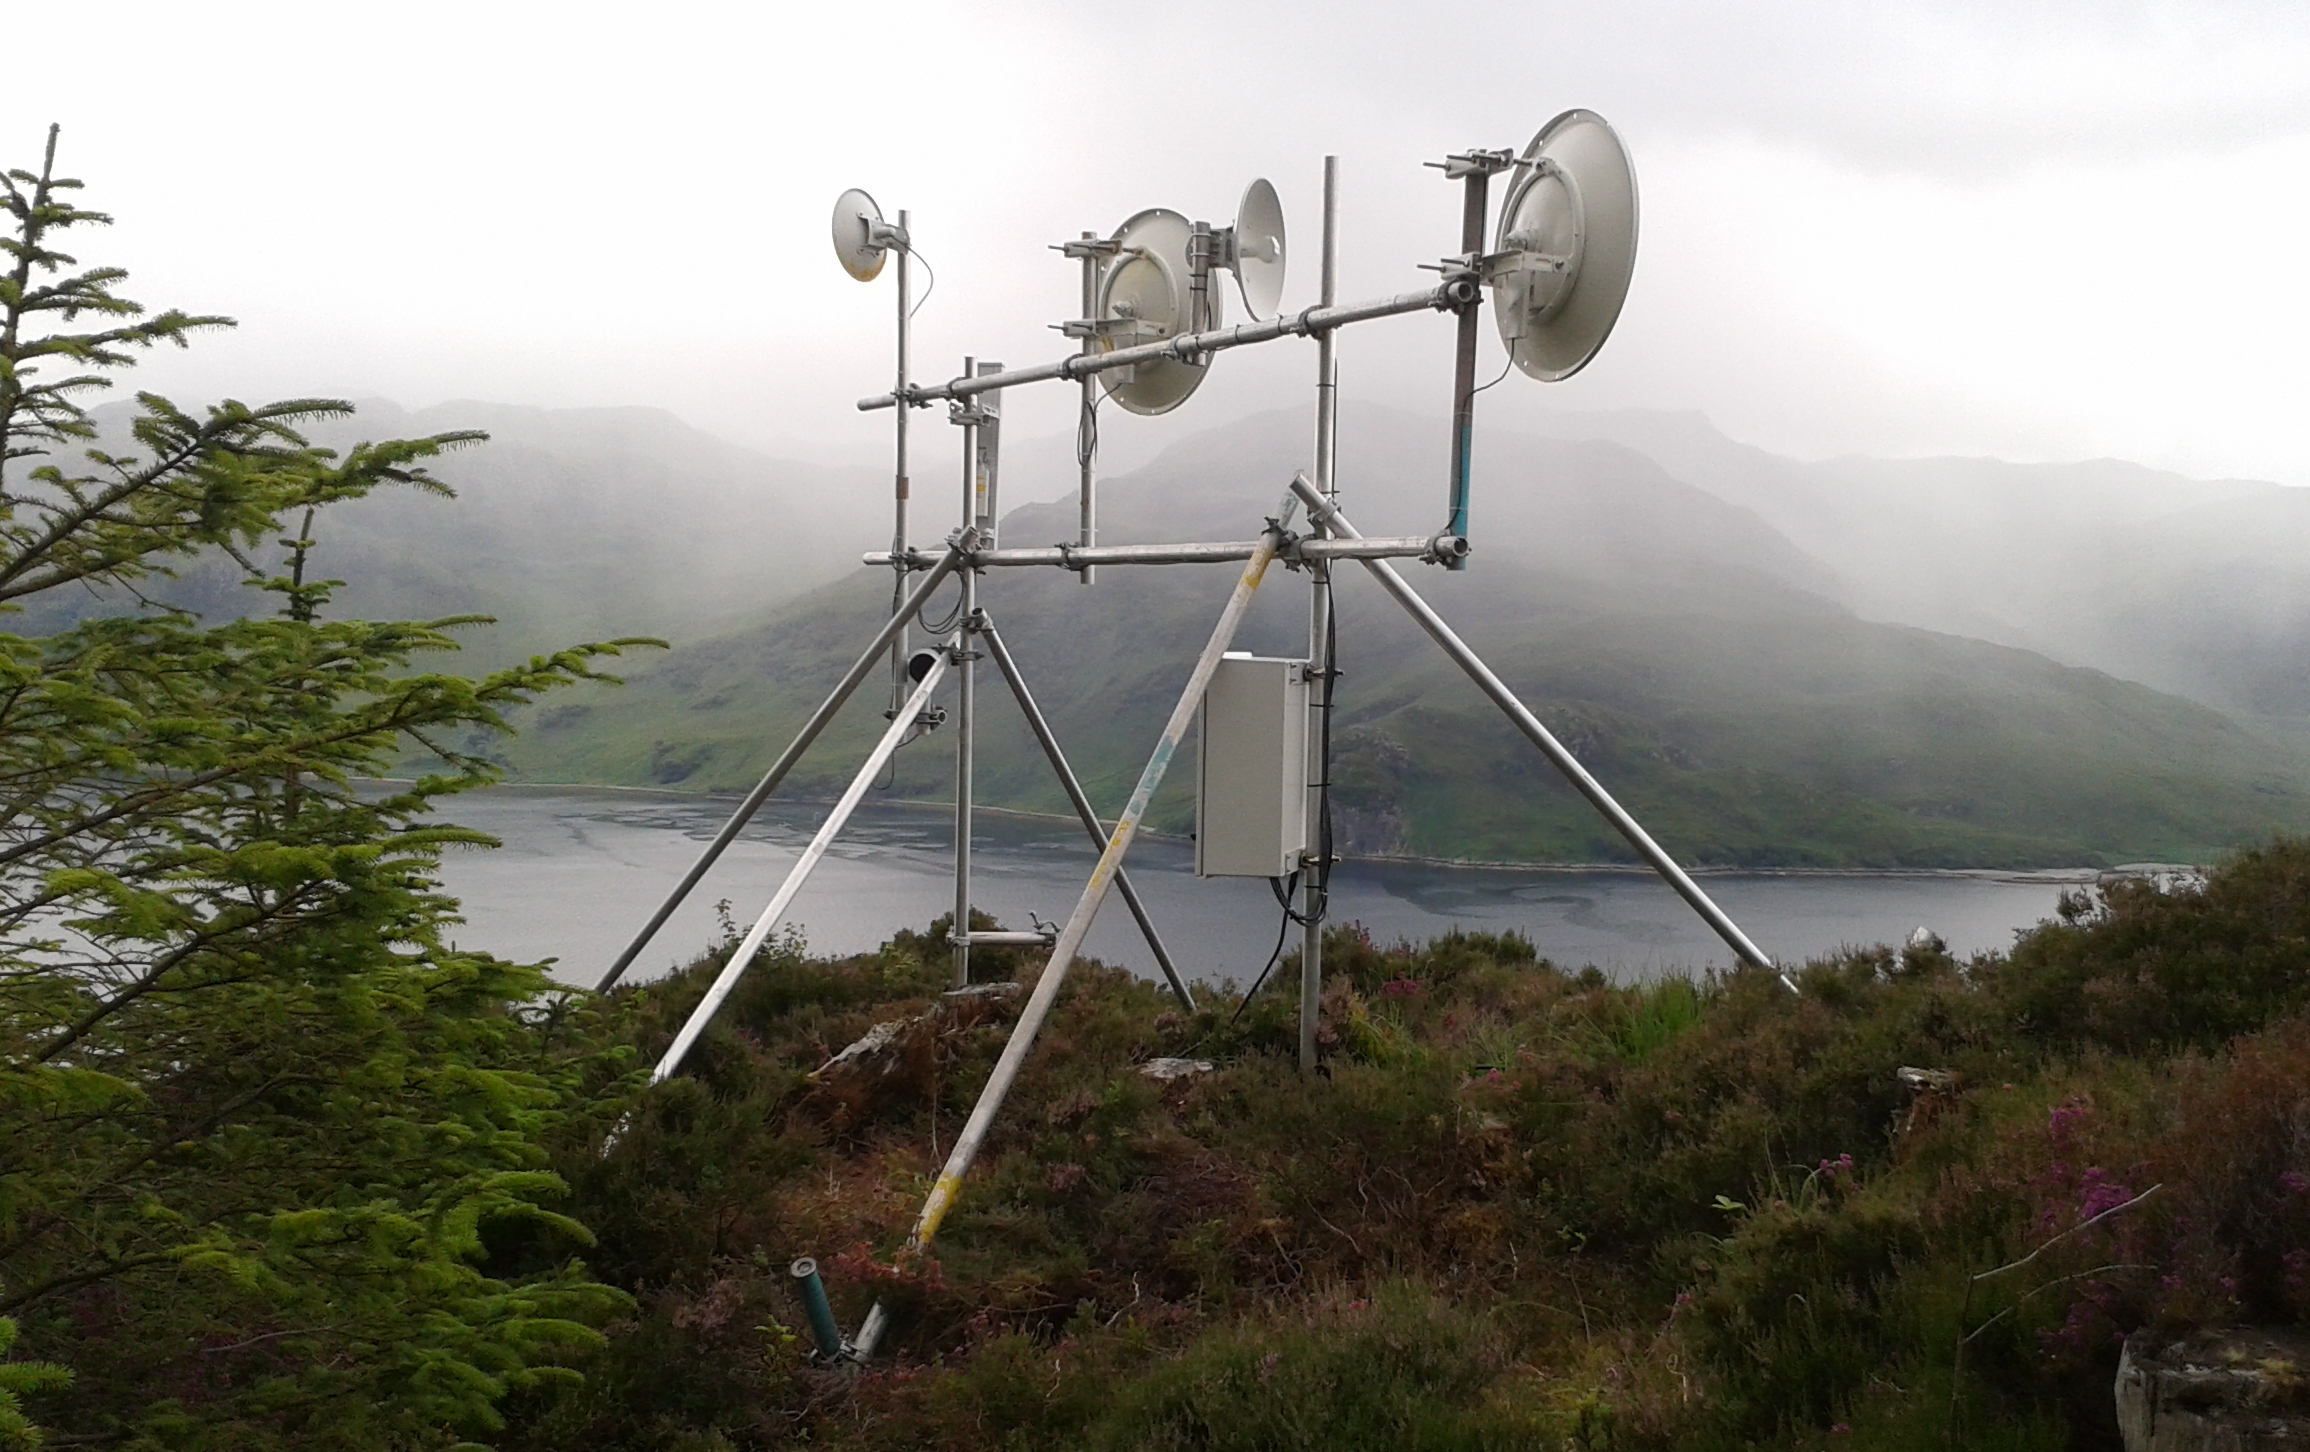
\includegraphics[width=\columnwidth]{figs/mhialairigh-from-behind}
 \caption{A basic relay}
\label{fig:mhialairigh}
\end{figure}

Recently, it has become possible to obtain adequate bandwidth at two major exchanges, but the cost is only reasonable if communities combine and buy at ``bulk'' prices.  For this one needs two things: an organization -- a co-operative -- that will act on behalf of the communities to obtain the economies of scale and a networking infrastructure

The terrain and the sociology of the Highlands and Island raises some important issues for both of these.
\todo[inline]{First bullet point below is very long and visually disturbing in comparison to the others.  Peter: I don't like footnotes, but maybe they cause less visual offence.  If space is a problem, take it out.}
\begin{itemize} 
\item The social communities do not always align well with the ``electronic'' communities. It is relatively easy to bounce signals back and forth across a loch or glen, but extremely hard to carry them over a 1000m high range of mountains. The reasons for this are social and economic and sometimes determined by the ways in which communities obtain funding\footnote{Knoydart is an isolated peninsula (see Fig.~\ref{fig:whixmap})  of which the North and West coasts are served by a network based on Loch Hourn and the South coast is served by Loch Nevis.  Contrast this with the Sleat peninsula which could, rationally,  be split into three sections, served by Loch Hourn, Loch Nevis and Eigg, but is run independently as a single entity with three connections to the rest of the world.}.
\item Communities structure their networks in various ways, and the complexity varies from a single point-to multipoint distribution system to a network with six relays  eight or more point-to-point links.  In some cases the networks have more than one physical path between relays for redundancy.
\item Many adjacent communities have successfully duplicated the local access network model. Together they cover a significantly large, contiguous geographical area. 
\item Communities may temporarily share resources (links or backhaul) when appropriate but this is not done in a systematic or organised fashion.
\end{itemize}
Stimulated in part by developments in the Highlands and Islands, communities in the Scottish Borders South of Edinburgh started  to develop similar networks.  While the terrain is also mountainous, the communities are within 40km of Edinburgh where fibre services are available.   However these are only affordable if the communities combine to purchase bandwidth at scale. To this end a community interest company, HUBS, was established whose members are the communities itself.  In addition to backhaul, HUBS provides technical help and other services.  It is anticipated that HUBS will extend its reach to serve the West Coast and achieve further economies of scale, for example in the puchase of transit.
